%=============================================================================
% Budget-Constrained Conformal Risk Control for Fraud Decisioning under Drift
% and Endogenous Label Arrival.
%
% ONE self-contained file. No .bib, no external figures, no \input.
% Compiles on Overleaf with pdflatex alone.
% Flip the toggle below from anonfalse to anontrue for a double-blind build.
%=============================================================================
\documentclass[conference]{IEEEtran}
\IEEEoverridecommandlockouts

\newif\ifanon
\anonfalse

\usepackage{amsmath}
\usepackage{amssymb}
\usepackage{booktabs}
\usepackage{graphicx}
\usepackage{algorithm}
\usepackage{algorithmic}
\usepackage{url}
\usepackage{tikz}
\usepackage{pgfplots}
\pgfplotsset{compat=1.18}
\usetikzlibrary{arrows.meta,positioning,calc,fit,backgrounds,decorations.pathreplacing}

\newtheorem{proposition}{Proposition}
\newtheorem{assumption}{Assumption}
% IEEEtran carries no proof environment and amsthm fights it; define one.
\newenvironment{proof}{\par\noindent\textit{Proof sketch.}\ }{\hfill$\blacksquare$\par\medskip}

\definecolor{cA}{RGB}{31,90,150}
\definecolor{cB}{RGB}{200,90,20}
\definecolor{cC}{RGB}{20,130,80}
\definecolor{cD}{RGB}{150,40,60}

\pgfplotsset{
  tinyplot/.style={
    width=0.96\columnwidth, height=4.55cm,
    tick align=outside,
    tick label style={font=\scriptsize},
    label style={font=\scriptsize},
    legend style={font=\scriptsize, draw=none, fill=none, inner sep=1pt},
    every axis plot/.append style={line width=0.6pt},
  }
}

% >>> INLINE-DATA BEGIN (generated by tools/make_paper_data.py; do not edit)
% ---------------------------------------------------------------------------
% Generated by tools/make_paper_data.py from results/results.json.
% Do not hand-edit: run `make paper-data` to rebuild and re-splice.
% source commit 8de870cbcf55102bad1d7ed6d1defe49cfa8719c  generated 2026-09-04T22:38:01Z
% ---------------------------------------------------------------------------

% TABLE I body: methods on SynB2B-Fraud-Stream
\newcommand{\TableMethodsBody}{%
M0 \textsc{static} & 0.02481 & 0.01737 & 0.04868 & 0.01997 & 0 & 226218 & -- \\
M1 \textsc{conf-fixed} & 0.02481 & 0.01737 & 0.04868 & 0.01997 & 0 & 226218 & -- \\
M2 \textsc{cost-thresh} & 0.01947 & 0.01124 & 0.02469 & 0.01945 & 0.922 & 160221 & 0.116 \\
M3 \textsc{aci-budget} & 0.01997 & 0.01228 & 0.02499 & 0.01908 & 0.284 & 164709 & 0.0888 \\
M4 \textsc{aci-budget-crc} & 0.02011 & 0.01217 & 0.02541 & 0.01911 & 0.305 & 167382 & 0.0533 \\
\textbf{M5 \textsc{-iap}} & 0.02068 & 0.01242 & 0.02287 & 0.01848 & 0.321 & 173129 & 0.877 \\
\quad M5, oracle $p_d$ & 0.02114 & 0.01269 & 0.02235 & 0.01816 & 0.211 & 178423 & 1.09 \\
}

% TABLE II body: exploration ablation on SynB2B-Fraud-Stream (M5)
\newcommand{\TableEpsBody}{%
0 & 0 & 0.866 & [0.840, 0.893] & 0.01231 & 0.02697 & 172510 \\
0.0500 & 69 & 0.870 & [0.846, 0.895] & 0.01236 & 0.02715 & 172724 \\
0.120 & 168 & 0.877 & [0.854, 0.903] & 0.01242 & 0.02734 & 173129 \\
0.250 & 356 & 0.894 & [0.875, 0.914] & 0.01252 & 0.02786 & 173429 \\
0.400 & 572 & 0.927 & [0.906, 0.948] & 0.01264 & 0.02856 & 174172 \\
0.600 & 870 & 0.971 & [0.951, 0.991] & 0.01287 & 0.02981 & 175379 \\
0.800 & 1196 & 0.954 & [0.893, 1.01] & 0.01377 & 0.03365 & 178900 \\
}

% TABLE III body: external validity, ULB card portfolio
\newcommand{\TableUlbBody}{%
M0 \textsc{static} & 0.0009484 & 0.0003289 & 0.02384 & 0.01811 & 0 & 377.7 & -- \\
M2 \textsc{cost-thresh} & 0.0008995 & 0.0003083 & 0.02075 & 0.01822 & 0.362 & 487.6 & 0.602 \\
M4 \textsc{aci-budget-crc} & 0.0009530 & 0.0003329 & 0.02057 & 0.01798 & 0.0198 & 392.8 & 0.785 \\
\textbf{M5 \textsc{-iap}} & 0.0009070 & 0.0003081 & 0.02058 & 0.01822 & 0.341 & 489.5 & 0.903 \\
}

% FIGURE 3: realised risk on the auto-allow path, per 2000-transaction block
\newcommand{\SeriesMone}{(138.467,0.010874) (147.32,0.0105859) (156.199,0.0126049) (164.827,0.0155361) (173.169,0.00816218) (181.605,0.0080897) (189.839,0.00852249) (197.989,0.00765206) (206.083,0.00323789) (213.96,0.0101829) (221.938,0.00701744) (230.093,0.00946774) (238.04,0.0107339) (245.913,0.00745152) (253.85,0.00775767) (261.711,0.00875181) (269.624,0.00635495) (277.412,0.0064606) (285.427,0.00574383) (293.149,0.0110736) (300.703,0.0146436) (308.315,0.0136246) (315.996,0.0360243) (323.629,0.0412245) (331.093,0.0401144) (338.558,0.037024) (345.861,0.0435648) (353.192,0.0369149) (360.685,0.0423367) (368.202,0.0407471) (375.57,0.0150259) (384.2,0.019953) (393.832,0.146021) (404.401,0.0332698) (416.738,0.0232669) (431.091,0.0191029) (448.124,0.0279089) (468.244,0.0355294) (493.52,0.0554749) (523.88,0.0947877)}
\newcommand{\SeriesMfour}{(138.467,0.010874) (147.32,0.0105859) (156.199,0.0112692) (164.827,0.0103539) (173.169,0.00553455) (181.605,0.00757995) (189.839,0.00807153) (197.989,0.00757698) (206.083,0.00335472) (213.96,0.0101781) (221.938,0.00563596) (230.093,0.0095428) (238.04,0.0105609) (245.913,0.00662186) (253.85,0.0064381) (261.711,0.00749554) (269.624,0.00597689) (277.412,0.00599265) (285.427,0.00506611) (293.149,0.00983985) (300.703,0.0127078) (308.315,0.011654) (315.996,0.0353583) (323.629,0.0381199) (331.093,0.0355524) (338.558,0.033226) (345.861,0.0413617) (353.192,0.0339877) (360.685,0.0394595) (368.202,0.0365476) (375.57,0.0122255) (384.2,0.0145786) (393.832,0.139947) (404.401,0.0288502) (416.738,0.0130065) (431.091,0.0133892) (448.124,0.0162001) (468.244,0.0214636) (493.52,0.0316125) (523.88,0.0526075)}
\newcommand{\SeriesMfive}{(138.467,0.0108228) (147.32,0.0107897) (156.199,0.0118996) (164.827,0.0135113) (173.169,0.00716188) (181.605,0.00680963) (189.839,0.00760101) (197.989,0.00740838) (206.083,0.00305598) (213.96,0.00913973) (221.938,0.0056993) (230.093,0.00958729) (238.04,0.010591) (245.913,0.00699592) (253.85,0.00651491) (261.711,0.00821439) (269.624,0.00600709) (277.412,0.0060414) (285.427,0.00519324) (293.149,0.0102334) (300.703,0.0134135) (308.315,0.0120907) (315.996,0.0362102) (323.629,0.0415039) (331.093,0.0381285) (338.558,0.0351377) (345.861,0.0431665) (353.192,0.0345051) (360.685,0.0396263) (368.202,0.0364234) (375.57,0.0118209) (384.2,0.0144967) (393.832,0.140144) (404.401,0.0288991) (416.738,0.0130869) (431.091,0.0134365) (448.124,0.0164439) (468.244,0.0218279) (493.52,0.0320204) (523.88,0.0529326)}
\newcommand{\AlphaSynb}{0.0124}
\newcommand{\DriftA}{227.59}
\newcommand{\DriftB}{312.27}
\newcommand{\DriftC}{388.94}

% FIGURE 4: review budget against realised risk (M5), with bootstrap band
\newcommand{\BudgetCurve}{(0.0075,0.0132214) (0.0125,0.0128747) (0.02,0.0124211) (0.03,0.0119708) (0.045,0.0114339)}
\newcommand{\BudgetLo}{(0.0075,0.0129367) (0.0125,0.0125698) (0.02,0.0120909) (0.03,0.0116313) (0.045,0.0110591)}
\newcommand{\BudgetHi}{(0.0075,0.0134834) (0.0125,0.0131479) (0.02,0.0127325) (0.03,0.0122972) (0.045,0.0117935)}
\newcommand{\BudgetBand}{(0.0075,0.0129367) (0.0125,0.0125698) (0.02,0.0120909) (0.03,0.0116313) (0.045,0.0110591) (0.045,0.0117935) (0.03,0.0122972) (0.02,0.0127325) (0.0125,0.0131479) (0.0075,0.0134834)}
\newcommand{\BudgetOverall}{(0.0075,0.0212233) (0.0125,0.0209738) (0.02,0.0206795) (0.03,0.0203358) (0.045,0.0197767)}
\newcommand{\BudgetInfeas}{(0.0075,0.335) (0.0125,0.327031) (0.02,0.32125) (0.03,0.315156) (0.045,0.268125)}

% FIGURE 5: where the calibration weight comes from, over time (M5)
\newcommand{\CompReview}{(161.722,0.0461811) (165.859,0.0395554) (171.093,0.0335109) (176.333,0.0298812) (181.532,0.0274877) (186.765,0.0261391) (191.851,0.0252705) (196.928,0.0241437) (202.055,0.0233753) (207.083,0.0228509) (212.046,0.0223236) (216.932,0.0222444) (221.901,0.0219871) (226.978,0.0216513) (232.184,0.0218052) (237.033,0.02248) (241.003,0.0214634) (245.842,0.0220946) (250.889,0.0212459) (255.786,0.0214005) (260.75,0.0212237) (265.703,0.0208096) (270.676,0.020637) (275.528,0.0203345) (280.345,0.0202826) (285.493,0.0201039) (290.262,0.0199138) (295.006,0.0196618) (299.758,0.019552) (304.482,0.0195396) (309.338,0.0193947) (313.145,0.0192397) (317.891,0.0190248) (322.679,0.0185432) (327.406,0.0182864) (331.996,0.0186027) (336.73,0.0182943) (341.257,0.0183724) (345.96,0.0183952) (350.432,0.0184129) (355.049,0.0185576) (359.686,0.0185015) (364.565,0.0183126) (369.162,0.0185151) (373.618,0.0185119) (378.52,0.018677) (382.989,0.018502) (388.928,0.0182486) (395.226,0.0181805) (401.586,0.0180473) (408.769,0.018073) (416.789,0.0179179) (425.355,0.0174122) (435.066,0.0170926) (445.709,0.017168) (457.313,0.0168888) (470.943,0.0169861) (486.686,0.0167553) (504.067,0.0169489) (523.564,0.0169954) (561.345,0.0168783)}
\newcommand{\CompLedger}{(161.722,0.949526) (165.859,0.956616) (171.093,0.962839) (176.333,0.966627) (181.532,0.96921) (186.765,0.970702) (191.851,0.971532) (196.928,0.97278) (202.055,0.973593) (207.083,0.974146) (212.046,0.974717) (216.932,0.974853) (221.901,0.975129) (226.978,0.975502) (232.184,0.975416) (237.033,0.974852) (241.003,0.97599) (245.842,0.975412) (250.889,0.976387) (255.786,0.976274) (260.75,0.976501) (265.703,0.976961) (270.676,0.977105) (275.528,0.977395) (280.345,0.97742) (285.493,0.977627) (290.262,0.97782) (295.006,0.978048) (299.758,0.97816) (304.482,0.978163) (309.338,0.978278) (313.145,0.978439) (317.891,0.978672) (322.679,0.979135) (327.406,0.979385) (331.996,0.979053) (336.73,0.97934) (341.257,0.979217) (345.96,0.979211) (350.432,0.979206) (355.049,0.979051) (359.686,0.979124) (364.565,0.979327) (369.162,0.979119) (373.618,0.979119) (378.52,0.978965) (382.989,0.979145) (388.928,0.979412) (395.226,0.979486) (401.586,0.979657) (408.769,0.97964) (416.789,0.979784) (425.355,0.980281) (435.066,0.980592) (445.709,0.980484) (457.313,0.980772) (470.943,0.980626) (486.686,0.980842) (504.067,0.980644) (523.564,0.980593) (561.345,0.980799)}
\newcommand{\CompExplore}{(161.722,0.00429323) (165.859,0.00382822) (171.093,0.00365055) (176.333,0.00349166) (181.532,0.00330206) (186.765,0.00315847) (191.851,0.00319763) (196.928,0.00307586) (202.055,0.00303165) (207.083,0.0030027) (212.046,0.00295958) (216.932,0.00290264) (221.901,0.00288401) (226.978,0.00284642) (232.184,0.00277846) (237.033,0.00266837) (241.003,0.00254699) (245.842,0.00249296) (250.889,0.00236677) (255.786,0.00232565) (260.75,0.00227521) (265.703,0.00222905) (270.676,0.00225778) (275.528,0.00227076) (280.345,0.00229735) (285.493,0.0022689) (290.262,0.0022663) (295.006,0.00229039) (299.758,0.00228754) (304.482,0.0022972) (309.338,0.0023276) (313.145,0.00232142) (317.891,0.00230281) (322.679,0.00232145) (327.406,0.00232821) (331.996,0.00234453) (336.73,0.00236581) (341.257,0.00241072) (345.96,0.00239342) (350.432,0.00238084) (355.049,0.00239141) (359.686,0.00237494) (364.565,0.00235986) (369.162,0.00236592) (373.618,0.00236906) (378.52,0.00235802) (382.989,0.00235321) (388.928,0.00233986) (395.226,0.00233309) (401.586,0.00229585) (408.769,0.00228676) (416.789,0.00229759) (425.355,0.00230672) (435.066,0.00231534) (445.709,0.00234819) (457.313,0.00233884) (470.943,0.00238812) (486.686,0.00240316) (504.067,0.00240721) (523.564,0.00241199) (561.345,0.00232261)}

% estimator reading against the truth of the same window (M4 and M5)
\newcommand{\EstMfour}{(162.787,0.0124) (168.881,0.0124) (176.333,0.0124) (183.705,0.0124) (189.899,0.0124) (196.928,0.0124) (204.119,0.0124) (209.943,0.0124) (216.932,0.0124) (224.001,0.0124) (231.113,0.0124) (237.033,0.115675) (243.988,0.283753) (250.889,0.292008) (256.733,0.322853) (263.673,0.330382) (270.676,0.335615) (276.461,0.38545) (283.409,0.387158) (290.262,0.400408) (296.929,0.397963) (302.5,0.432656) (309.338,0.476247) (315.913,0.19117) (321.745,0.264548) (328.327,0.00083204) (334.909,0.323526) (341.257,0.134998) (346.834,0.0729689) (353.179,0.456652) (359.686,0.571509) (365.382,0.558054) (371.863,0.680264) (378.52,0.73012) (385.356,0.775287) (393.788,0.794798) (402.848,0.802583) (413.51,0.5174) (423.513,0.257415) (437.253,0.149005) (452.559,0.102066) (467.692,0.0782369) (489.921,0.0554365) (515.382,0.0438814) (561.345,0.0393571)}
\newcommand{\EstMfive}{(161.722,0.00998507) (167.842,0.0114592) (175.248,0.0104632) (182.593,0.0124908) (188.86,0.0123358) (195.924,0.011559) (203.078,0.0120455) (209.943,0.0123026) (215.919,0.0123808) (222.91,0.0115798) (230.146,0.0109096) (237.033,0.0104881) (243.115,0.0105531) (249.833,0.0109442) (256.733,0.0110286) (262.704,0.0111235) (269.703,0.0113296) (276.461,0.0110809) (283.409,0.0107708) (289.324,0.010529) (295.961,0.0105155) (302.5,0.0103113) (309.338,0.0101917) (314.985,0.0102607) (321.745,0.0102737) (328.327,0.0102773) (333.942,0.0105053) (340.443,0.0132101) (346.834,0.0140408) (353.179,0.0153166) (358.697,0.0166983) (365.382,0.0182479) (371.863,0.0204896) (378.52,0.0219897) (385.356,0.0240442) (393.788,0.0242045) (402.848,0.0249815) (411.781,0.0312653) (423.513,0.0348072) (437.253,0.0342751) (452.559,0.0340178) (467.692,0.0341591) (489.921,0.0354046) (515.382,0.0360668) (561.345,0.0423928)}
\newcommand{\EstTrue}{(161.722,0.00967099) (167.842,0.00977842) (175.248,0.0100315) (182.593,0.00912875) (188.86,0.00867524) (195.924,0.00881656) (203.078,0.00863773) (209.943,0.00815765) (215.919,0.00834875) (222.91,0.00806143) (230.146,0.00803978) (237.033,0.00820484) (243.115,0.00820112) (249.833,0.00804369) (256.733,0.00793977) (262.704,0.00787088) (269.703,0.00779818) (276.461,0.00775114) (283.409,0.00760998) (289.324,0.00746595) (295.961,0.00762176) (302.5,0.00774833) (309.338,0.00801815) (314.985,0.00875881) (321.745,0.0102153) (328.327,0.0116361) (333.942,0.0126679) (340.443,0.0137699) (346.834,0.0149584) (353.179,0.0157078) (358.697,0.0165747) (365.382,0.0174741) (371.863,0.0183518) (378.52,0.0184016) (385.356,0.0186569) (393.788,0.0219304) (402.848,0.0267137) (411.781,0.0268485) (423.513,0.026641) (437.253,0.0265076) (452.559,0.0266626) (467.692,0.0269123) (489.921,0.0272267) (515.382,0.0288078) (561.345,0.0348715)}

% scalars quoted in captions
\newcommand{\NSeeds}{20}
\newcommand{\NBoot}{10{,}000}
\newcommand{\BudgetVal}{0.0200}
\newcommand{\HoldCap}{0.0800}
\newcommand{\EpsDefault}{0.120}
\newcommand{\AlphaUlb}{0.000930}
% <<< INLINE-DATA END

\title{Budget-Constrained Risk Calibration for\\Fraud Decisioning under Drift and
Endogenous Label Arrival}

\ifanon
\author{\IEEEauthorblockN{Author names withheld for review}
\IEEEauthorblockA{Affiliation withheld for review}}
\else
\author{\IEEEauthorblockN{Abhishek Sharma} \IEEEauthorblockA{\textit{Senior Member,
IEEE}\\ORCID 0009-0007-1103-2103}}
\fi

\begin{document}
\maketitle

\begin{abstract}
Fraud scores are not decisions. An accounts-payable team releases a payment, holds it
for dual-control approval, or routes it to an analyst, and the queue that receives it
has a fixed size. This work wraps a frozen scorer in a selective-decision layer
targeting the false-omission rate on auto-released traffic under a hard review budget.
The awkward part is that the policy chooses which labels it will ever see. Reviewed
items come back adjudicated within hours, an allowed fraud is recorded only if a
dispute or a reconciliation exception surfaces, and held items are never labelled.
Calibration data therefore piles up in the review band, at mid score, while the
quantity being tracked lives in the low-score tail. We give a feasibility condition
relating target, budget and score law, and an identification result for what random
exploration buys. On a 100,000-invoice B2B stream carrying three injected drift
events, an uncorrected estimator reads auto-release risk high by a factor of 18.8 over
matured windows. Arrival-propensity reweighting with a 0.120 exploration allocation
moves the truth-to-estimate ratio to 0.877 [0.854, 0.903]. Realised risk does not
improve, and what the correction buys is a believable estimate and a feasibility
signal that scores 0.898 balanced accuracy against an oracle, not less fraud.
\end{abstract}

\begin{IEEEkeywords}
conformal prediction, risk control, fraud detection, concept drift, selective
classification, delayed labels, B2B payments
\end{IEEEkeywords}

\section{Introduction}

A fraud model returns a number. Nobody pays a number. Downstream of the score a
payment is released, parked for dual-control approval, or dropped into an analyst's
queue whose size was fixed by headcount and an SLA long before anyone trained the
model. Risk lands in that decision layer, which in most shops is a pair of thresholds
somebody moved last quarter.

Conformal prediction is the obvious tool, since it turns a score into a finite-sample
guarantee and asks almost nothing of the model that produced it. Applying it here runs
into a constraint most of that literature leaves out: the abstention region has a hard
capacity, because analysts cost money and a payments organisation employs a countable
number of them. Active risk-controlling prediction
sets do budget labels~\cite{xu2024active}, but they budget queries to an oracle rather
than an operational queue that also decides the outcome.

There is a second constraint, and it is the one this paper is about. The policy
chooses its own labels. An item sent to review comes back adjudicated within hours. An item released is labelled only if something surfaces, a chargeback representment or
a three-way match that fails at reconciliation, and on invoice fraud that takes 30 to
180 days when it happens at all.
An item held for dual-control approval is never labelled. So the calibration set is dominated by review-band items,
which sit at mid score by construction, while the risk being tracked lives in the low-
score tail.

This is not staleness. It is bias, and filtering the window by arrival time does not
repair it, because the items that never arrive are the ones the guarantee is about.
Tighten the budget and calibration starves where it is needed most, while the estimate
stays flat and every detector watching the score distribution stays quiet.

Four things follow. A feasibility condition, an equivalence under three assumptions,
for when a target and a review budget can hold together. A minimum-exploration
argument in two parts, of which the identification half survives and the rate half
does not. A data extension, SynB2B-Fraud-Stream, annotating a published benchmark with
three drift events and an action-dependent arrival process, studied over two streams,
six methods and five seeds. And a measurement of how wrong the naive estimator gets.

\section{Related Work}

Concurrent work by Deng~\cite{deng2026} asks when fraud operations may authorize
automation at all, under shared analyst capacity, with finite-sample risk control on
three public corpora. That framework is not conformal and recalibrates nothing online. It does treat labels as selective and delayed, and shows action risk is unidentified
without restricting label evolution, but closes that gap with mature randomized audits
and a prespecified transport condition rather than by modelling disclosure. Here an
undisclosed release is not missing but booked clean, and thresholds recalibrate online
against an estimated arrival mechanism.

The calibration machinery is borrowed rather than invented. Split and inductive
conformal prediction supply the finite-sample statement~\cite{vovk2005,
papadopoulos2002}, and Gibbs and Cand\`es replace the fixed quantile with an online
recursion that adapts under shift and then under arbitrary shifts~\cite{gibbs2021,
gibbs2024}. Conformal risk control generalises coverage to any monotone
risk~\cite{angelopoulos2024}, with risk-controlling prediction sets as the batch
antecedent~\cite{bates2021}. Feldman and colleagues give the online version this
policy runs~\cite{feldman2022}. Barber and colleagues establish what survives when
exchangeability fails, which on a card portfolio it does within
hours~\cite{barber2023}, and a PID formulation adds integral and derivative terms to
the same update~\cite{angelopoulos2023}.

Selective classification supplies the abstention vocabulary~\cite{geifman2017,
geifman2019} and learning to defer the cost of routing to a human~\cite{mozannar2020};
neither caps how often the human may be asked. Active, anytime-valid risk-controlling
prediction sets do, under a fixed label budget~\cite{xu2024active}. There the budget
governs which labels are purchased, whereas here the same queue purchases the label
and executes the decision, so spending it changes the outcome as well as the evidence.
Cost-sensitive conformal prediction with human-in-the-loop abstention trades review
cost against error in a soft objective~\cite{singh2026}, and Selective Conformal Risk
Control certifies risk after selection on exchangeable data, again with no
budget~\cite{xu2026}.

Online shift detection with conformal adaptation is the nearest prior art to the audit
protocol, and it monitors: no actions, no capacity, no path from the decision back
into the data~\cite{leong2026}. Audited conformal prediction~\cite{zhou2026} and
anytime-valid risk control~\cite{hultberg2026} tighten what a running system can
certify. Delayed and partial fraud feedback were documented a decade ago~\cite{dalpozzolo2014,
dalpozzolo2018}, and recent work formalises the limits that delayed, censored and
corrupted feedback impose in card networks~\cite{dhama2026a}, recovers labels causally
in payment graphs~\cite{dhama2026b}, folds corrupted feedback into online conformal
prediction~\cite{wang2026}, and names the general obstacle as the selective-labels
problem, where a decision that suppresses an outcome suppresses the evidence about
it~\cite{lakkaraju2017}.

\section{Problem Formulation}
\label{sec:prob}

Transactions arrive in time order. Transaction $t$ carries features $x_t$, an invoice
amount $v_t$ and a label $y_t \in \{0,1\}$ that may or may not ever be observed. A
scorer $s(\cdot)$, trained once and then frozen, emits $s_t = s(x_t)$. The policy
holds two thresholds $\tau^t_{\mathrm{lo}} \le \tau^t_{\mathrm{hi}}$ and maps the score
to an action,
\begin{equation}
a_t =
\begin{cases}
\textsf{allow} & s_t \le \tau^t_{\mathrm{lo}}\\
\textsf{hold} & s_t > \tau^t_{\mathrm{hi}}\\
\textsf{review} & \text{otherwise.}
\end{cases}
\end{equation}
The controlled quantity is the false-omission rate on auto-released traffic,
$R_t = \Pr(y = 1 \mid a = \textsf{allow})$ over a trailing window, and the requirement
is $R_t \le \alpha$. Review capacity is a hard cap: the share of traffic reaching an
analyst may not exceed $b$. Held volume is capped at $\beta$, which in accounts payable
is a working-capital limit rather than a risk limit, since a hold delays a supplier
payment and delayed suppliers stop shipping.

The filtration is where this departs from the usual setup. Write $Y_i$ for the latent
fraud state, $A_i$ for the label-arrival time, and $\widetilde{Y}_i$ for what the
ledger finally records, which is not always $Y_i$. A reviewed item returns
$\widetilde{Y}_i = Y_i$ within hours. A held item returns nothing, ever. On the
release path a fraud surfaces with probability $p_d(x_i)$, a legitimate payment never
surfaces, and whatever has not surfaced by the 180-day close is booked clean. Writing
$D_i \sim \mathrm{Bern}(p_d(x_i))$ for that disclosure draw, independent of $Y_i$
given $x_i$,
\begin{equation}
\label{eq:obs}
\widetilde{Y}_i = Y_i D_i \qquad \text{on the release path.}
\end{equation}
An undisclosed fraud is therefore not a missing row. It is a row recorded as good. The
calibration set at time $t$ is $\mathcal{C}_t = \{ i < t : A_i \le t \}$, and $A_i$ and
$\widetilde{Y}_i$ both depend on $a_i$, which the policy chose. So $\mathcal{C}_t$ is
not a sample of the past. It is the past, filtered through the policy's own decisions,
and the filter is tightest exactly where the estimate is needed.

\section{Method}
\label{sec:method}

\subsection{Arrival model}

Three channels, one per action, all Gamma laws in shape-scale form and all times in
days. A reviewed item is adjudicated after $\mathrm{Gamma}(2, 0.4)$ and its label is
the truth. Only a fraud can surface on the release path: it does so with probability
$p_d(x)$, after $\min(\mathrm{Gamma}(2, 30), 180)$, which is why
\eqref{eq:obs} multiplies rather than merely delays. A legitimate release generates no
event at all and is booked clean at the 180-day close, as is any fraud that never
surfaced. That second half matters more than the delay, and an estimator that treats
absence as missingness will read the wrong sign off it. A held item is never
labelled.

\subsection{Inverse-arrival-propensity reweighting}

Let $\pi_i$ be the probability that $i$ has produced an informative label by now. On
the review path it is known by construction, since the policy chose the review and the
SLA is an operational fact. On the release path $\pi_i = p_d(x_i)F_G(t - t_i)$ with
$F_G$ the disclosure delay law, and $p_d$ must be estimated, which is where the
modelling risk sits. On that path the ledger shows only the product $r(x)p_d(x)$, so $p_d$ is recovered as
a ratio: $\hat{q}$ fitted on matured release rows, whose label is $\widetilde{Y}$,
over $\hat{r}$ fitted on the rows an analyst adjudicated, which is the review band
plus the exploration draw. Both are ridge logistic fits on the standardised amount and
the frozen score. Neither sees the fraud topology that actually drives disclosure, so
$\hat{p}_d$ is a marginal approximation, and the fit needs closed windows, which makes
the correction itself lagged. The estimate on a score grid is
\begin{equation}
\label{eq:est}
\widehat{R}_t(\tau) =
\frac{\sum_{i \in \mathcal{D}_t} w_i\,O_i\,\widetilde{Y}_i\,\pi_i^{-1}\,
      \mathbf{1}\{s_i \le \tau\}}
     {\sum_{i \in \mathcal{D}_t} w_i\,\mathbf{1}\{s_i \le \tau\}},
\end{equation}
where $\mathcal{D}_t$ is every decision taken in the window, held items aside, $O_i =
\mathbf{1}\{A_i \le t\}$, and $w_i = \rho^{\,t-t_i}\mathbf{1}\{\pi_i \ge \pi_0\}$. The
denominator counts decisions, not labels. Restricting it to arrived labels would be
outcome-selected, because a surfaced fraud arrives months before the close that books
an undisclosed one clean.
The propensity enters the numerator alone, inflating each surfaced fraud so that it
stands for the ones still sitting inside the reconciliation window and not yet visible
to anybody. Trimming at $\pi_0$ drops items from both sums, so \eqref{eq:est} targets the overlap
population $\{\pi_i \ge \pi_0\}$, exponentially weighted rather than the trailing-
window mean of Section~\ref{sec:prob}. That gap is measured: the estimand sits 0.07792 from the trailing-window risk in
relative terms, and trimming removes 0.1509 of rows carrying 0.1829 of their fraud.

\begin{figure}[t]
\centering
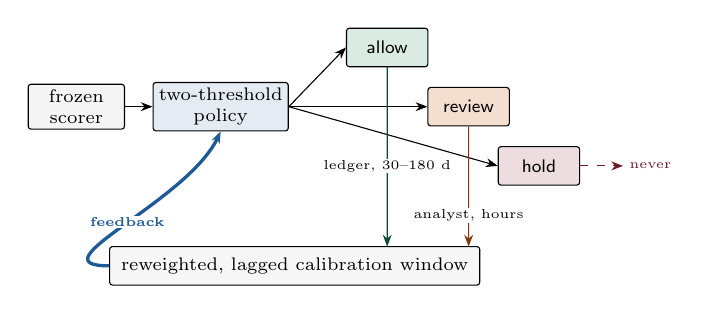
\begin{tikzpicture}[scale=0.94, transform shape,
  font=\scriptsize, >={Stealth[length=1.5mm]},
  box/.style={draw, rounded corners=1pt, align=center, inner sep=2.2pt,
              minimum height=5.2mm},
  act/.style={box, minimum width=11mm},
  lbl/.style={fill=white, inner sep=0.6pt, font=\tiny, text=black},
]
\node[box, fill=black!4, minimum width=13mm] (sc)  at (0.55, 0)     {frozen\\scorer};
\node[box, fill=cA!12, minimum width=17mm]   (pol) at (2.50, 0)     {two-threshold\\policy};
\node[act, fill=cC!16]                       (al)  at (4.75, 0.80)  {\textsf{allow}};
\node[act, fill=cB!20]                       (rv)  at (5.85, 0)     {\textsf{review}};
\node[act, fill=cD!16]                       (hd)  at (6.80,-0.80)  {\textsf{hold}};
\node[box, fill=black!3, minimum width=50mm] (cal) at (3.50,-2.15)
     {reweighted, lagged calibration window};
\draw[->] (sc) -- (pol);
\draw[->] (pol.east) -- (al.west);
\draw[->] (pol.east) -- (rv.west);
\draw[->] (pol.east) -- (hd.west);
\draw[->, cD!70!black, dashed] (hd.east) -- ++(0.58,0)
      node[right=-1pt, font=\tiny, text=cD!70!black] {never};
\draw[->, cC!60!black] (al.south) -- (4.75,-1.89)
      node[pos=0.55, lbl] {ledger, 30--180 d};
\draw[->, cB!65!black] (rv.south) -- (5.85,-1.89)
      node[pos=0.74, lbl] {analyst, hours};
\draw[->, very thick, cA] (cal.west) .. controls +(-1.05,0) and +(-0.45,-0.95) ..
      (pol.south) node[pos=0.52, lbl, text=cA] {\textbf{feedback}};
\end{tikzpicture}
\caption{The decision loop. Actions determine which labels ever reach the calibration
window, and the calibration window determines the next actions. The thick edge is the
dependence the rest of this paper is about; the dashed edge carries nothing, ever.}
\label{fig:sys}
\end{figure}

\subsection{Update, budget projection, infeasibility}

The recursion is the Gibbs--Cand\`es one, driven by the lagged, reweighted stream,
\begin{equation}
\alpha_{t+1} = \alpha_t + \gamma\,(\alpha - \mathrm{err}_t),
\end{equation}
with $\tau_{\mathrm{lo}}$ read off the reweighted curve, as a quantile (M3) or through
a conformal-risk-control threshold search over the same window (M4, M5). A candidate counts only if at least $200$ units of calibration weight sit at or below
it, since certifying a one-in-a-hundred risk from a dozen observations is small
arithmetic rather than conservatism. 

Capacity is enforced separately. Given $\tau_{\mathrm{lo}}$, the upper threshold
$\tau_{\mathrm{hi}}$ is placed by an online quantile so the band carries
$b(1-\varepsilon)$ of traffic, which stops the risk and capacity constraints fighting
over one knob, and a final projection caps the served load at $b$. When no admissible
$\tau_{\mathrm{lo}}$ meets $\alpha$ within that capacity, the policy widens the band
as far as $b$ allows and raises a \emph{budget-infeasible} flag. It does not quietly
miss the target and report success.

\subsection{Exploration}

A fraction $\varepsilon$ of review capacity is spent on transactions drawn uniformly
at random from below $\tau_{\mathrm{lo}}$, independent of score, which leaves
$R(\tau_{\mathrm{lo}})$ intact as the released region's risk. These are items the policy is already confident about, so the spend looks like waste
on any dashboard an operations manager reads, and that is why it gets cut first in
production. Their labels are the only ones drawn from the release region at a known
probability, so they alone anchor $\hat{r}$ there.

\subsection{When are the target and the budget compatible?}

Let $F$ be the score law, $r(u) = \Pr(y=1 \mid s = u)$ the conditional fraud rate and
$R(\tau) = \mathbb{E}[y \mid s \le \tau]$ the risk on everything released below
$\tau$. The argument needs three assumptions, and one is doing real work. (A1) $F$ is continuous and strictly
increasing on the operating range. (A2) $r$ is non-decreasing in the score. (A3) the
analyst queue is standing capacity and is always spent, so the band carries
$b(1-\varepsilon)$.

\begin{proposition}[Feasibility]
\label{prop:feas}
Under \emph{(A1)--(A3)}, with $0 \le \varepsilon \le 1$ and
$0 < b(1-\varepsilon) < 1-\beta$ so that $q := 1 - \beta - b(1-\varepsilon)$ lies in
$(0,1)$ and the release region is non-empty, the pair
$(\alpha, b)$ is jointly attainable if and only if
$R\!\left(F^{-1}(q)\right) \le \alpha$, equivalently
$\alpha \ge \alpha_{\min}(b) := R(F^{-1}(1 - \beta - b(1-\varepsilon)))$, and
$\alpha_{\min}$ is non-increasing in $b$.
\end{proposition}

\begin{proof}
Under (A3) the held mass is $1 - F(\tau_{\mathrm{lo}}) - b(1-\varepsilon)$, so $\beta$
forces $F(\tau_{\mathrm{lo}}) \ge q$. Under (A2) $R$ is non-decreasing: for $\tau_1 <
\tau_2$, $R(\tau_2)$ is a convex combination of $R(\tau_1)$ and $\mathbb{E}[y \mid
\tau_1 < s \le \tau_2]$, whose second term is at least $r(\tau_1) \ge R(\tau_1)$. The
smallest admissible release set is the one at $F^{-1}(q)$, feasible exactly when its
risk clears $\alpha$. Monotonicity in $b$ follows since $q$ decreases as $b$ grows.
\end{proof}

Drop (A2) and the condition stays sufficient, since $\tau_{\mathrm{lo}} = F^{-1}(q)$
is admissible whenever its risk clears $\alpha$. What it loses is necessity: with a
non-monotone $r$ a larger threshold can carry lower cumulative risk, so a pair can be
attainable while the condition reads false. The statement is also pointwise in the score law,
and under drift $F$ and $r$ move, so $\alpha_{\min}$ is a property of the current
regime rather than of the stream, and the implementation evaluates it per window on
the
\emph{estimated} $R$, which makes the flag worth exactly what the estimator is worth.

\begin{proposition}[Identification]
\label{prop:ident}
On the release path only $Z = Y \cdot D$ is observed, with
$D \sim \mathrm{Bern}(p_d(x))$ independent of $Y$ given $x$. Then
$\Pr(Z = 1 \mid x) = r(x)\,p_d(x)$, so for any $c(x)$ with
$p_d(x) \le c(x) \le 1/r(x)$ the pair $(cr,\; p_d/c)$ is again a rate-probability
pair and induces the same observable law. Only the product is identified from the
ledger channel.
\end{proposition}

The review band identifies $r$ on $(\tau_{\mathrm{lo}}, \tau_{\mathrm{hi}}]$, disjoint
from the release region, so it constrains $r$ there only through a functional-form
assumption. An exploration sample drawn from below $\tau_{\mathrm{lo}}$ at a known probability
identifies $r$ directly on that support. Then $p_d$ follows there, and only there. The honest reading is weaker
than the one we set out to prove: at $\varepsilon = 0$ release-path risk is not
nonparametrically identified, and point identification rests on an extrapolation no
data in that region can test.

We then asked how much exploration a rate guarantee needs. Bernstein's inequality on
the exploration sample, treating it as a fixed-window Bernoulli mean with $R \approx
\alpha$, gives $|\hat{R} - R| \le \eta\alpha$ with probability $1-\delta$ once
$n_{\exp} \ge 2[(1-\alpha) + \eta/3]\log(2/\delta)/(\eta^2 \alpha)$, and with $n_{\exp} \approx \varepsilon b L$ over a window of $L = 45000$,
\begin{equation}
\label{eq:eps}
\varepsilon \;\ge\; \frac{2\left[(1-\alpha) + \eta/3\right]\log(2/\delta)}
{\eta^{2}\,\alpha\,b\,L}.
\end{equation}
At $\eta = 1$, $\delta = 0.0500$ this asks for $n_{\exp} \ge 786$, that is
$\varepsilon \ge 0.873$, to pin the estimate within one target-width, and halving the tolerance demands 2748 items, an $\varepsilon$ of 3.05. The bound is vacuous, and it
bounds a fixed window rather than the adaptive procedure. We report the measured curve
instead.

%% Fig. 2 (score-axis band) cut under the Sec. VI-F order to fund the
%% observed-data model, the estimator and the hyperparameter table.


Every window emits four numbers for audit: the reweighted estimate, realised risk over
matured labels, review demand against $b$, and the flag. A policy whose estimate is
flat while its realised risk climbs is blind, and no detector watching only the score
distribution will say so.

\begin{algorithm}[t]
\caption{Budgeted conformal decisioning with exploration}
\label{alg:main}
\begin{algorithmic}[1]
\STATE \textbf{input} target $\alpha$, budget $b$, hold cap $\beta$, decay $\rho$,
step $\gamma$, exploration share $\varepsilon$
\STATE $\alpha_1 \leftarrow \alpha$;
  $\mathcal{D} \leftarrow \emptyset$; $\mathcal{C} \leftarrow \emptyset$
\FOR{each arriving transaction $t$}
  \STATE $s_t \leftarrow s(x_t)$
  \STATE append the decision to $\mathcal{D}$; admit to $\mathcal{C}$ every
      label with $A_i \le t$ \COMMENT{causal guard}
  \IF{$t \bmod m = 0$}
    \STATE $\hat{q},\hat{r} \leftarrow$ fits on matured $\mathcal{D}$ and
      adjudicated $\mathcal{C}$; $\hat{p}_d \leftarrow \hat{q}/\hat{r}$, clipped
    \STATE $\hat{R}(\cdot) \leftarrow$ \eqref{eq:est} over $\mathcal{D}$, using
      $O_i$ from $\mathcal{C}$, trimming $\pi_i < \pi_0$
    \STATE $\tau_{\mathrm{lo}} \leftarrow \max\{\tau : \hat{R}(\tau) \le \alpha_t\}$
    \IF{no such $\tau$ within $\beta$}
      \STATE widen to the cap and raise \textsf{infeasible}
    \ENDIF
    \STATE $\tau_{\mathrm{hi}} \leftarrow$ quantile giving band mass $b(1-\varepsilon)$
    \STATE $\alpha_{t+1} \leftarrow \alpha_t + \gamma(\alpha - \mathrm{err}_t)$
  \ENDIF
  \STATE $a_t \leftarrow$ action from $(s_t, \tau_{\mathrm{lo}}, \tau_{\mathrm{hi}})$
  \IF{$a_t = \textsf{allow}$ and $u_t < \varepsilon b / F(\tau_{\mathrm{lo}})$}
    \STATE $a_t \leftarrow \textsf{review}$ \COMMENT{exploration draw}
  \ENDIF
  \IF{$a_t = \textsf{review}$ and the window's $b$ slots are spent}
    \STATE $a_t \leftarrow$ automatic decision at the band midpoint
      \COMMENT{capacity projection}
  \ENDIF
  \STATE schedule $A_t$ from the channel implied by the served $a_t$
\ENDFOR
\end{algorithmic}
\end{algorithm}

\section{Experimental Setup}
\label{sec:setup}

The primary stream is SynB2B-Fraud~\cite{synb2b}, 100,000 buyer-to-supplier invoices
over 561.34 days with five fraud topologies, its statistics re-derived from the CSV:
1,500 fraudulent rows, 300 per topology, median invoice 3,492.66. Fraud is not
spread evenly in time, and the first 20\% of rows carries 0.385\% fraud against 1.78\%
over the rest, so a target calibrated on the training split would mean nothing. Targets are
stipulated instead.

We add two annotation layers, released as SynB2B-Fraud-Stream. Drift enters as a
second fraud channel layered on the generator's own labels, never as a relabelling, so
all 1,500 published labels survive: a covariate shift in the log-amount law, a 60-day
sign flip of the supplier-novelty coefficient, and a base-rate surge with a 9-day
half-life, magnitudes solved against stated targets rather than picked by eye.
Disclosure probabilities run from 0.86 for wire redirection down to 0.19 for
payment-term manipulation, because a redirected wire generates a phone call and a
manipulated payment term generates nothing. The ULB rows keep their original order and
are replayed on the same 561.34-day calendar, since 48 hours cannot carry a 180-day
reconciliation horizon.

The scorer is LightGBM, trained on the first 20\% in time order then frozen, isolating
the calibration layer from model staleness; it reaches AUC-PR 0.2049 and AUC-ROC
0.7313 over the rest. Over the ten days after each event AUC-PR falls by a
relative 0.7988 and 0.6805 for the covariate and concept shifts and \emph{rises} by
0.3233 after the prior shift, since a larger positive class makes average precision
easier. The second stream is the ULB card portfolio~\cite{dalpozzolo2018}. Cost constants are stipulated per stream and stated in the repository, and the claim made here concerns risk calibration, not cost optimality. The operating point is $\alpha = 0.0124$, $b = 0.0200$, $\beta = 0.0800$,
$\varepsilon = 0.120$, $\rho = 0.9975$, $\gamma = 0.018$, propensity floor
$\pi_0 = 0.0500$, a calibration window capped at 45000 items and 240 days, an update
every 250 transactions, and a support gate of 200 weight units. Costs are USD per thousand transactions. The controller is ACI- and CRC-inspired and
evaluated empirically: no theorem here covers the whole endogenous, delayed and
corrupted observation process, so no conformal guarantee is claimed for it. Intervals are percentile bootstraps over the five seed-level
replicates, which is the independent unit here; with five runs they are coarse and
should be read as exploratory rather than as tight confidence statements. Everything
runs on an Apple M4 Pro. Code, the full results file
and the decision log are at
\ifanon URL withheld for review\else \url{https://github.com/abhisheksharma2411/synb2b-fraud-stream}\fi.

\begin{table}[t]
\caption{Methods on SynB2B-Fraud-Stream, five seeds. FOR is the false-omission rate on
released traffic. ``dem.'' is review demand before the capacity projection and
``served'' is the analyst load after it, which is what the cap of $b=0.0200$ binds.
``Infeas.'' is the share of windows raising the budget-infeasibility flag. ``ratio''
is $\overline{R}_{\mathrm{true}}/\overline{R}_{\mathrm{est}}$, a quotient of two means
over matured windows, where $1$ is calibrated and smaller means the estimator reads
high. It is a calibration ratio, not a statistical bias.}
\label{tab:methods}
\centering\scriptsize
\setlength{\tabcolsep}{1.0pt}
\begin{tabular}{lrrrrrrr}
\toprule
Method & FOR & quiet & dem. & served & Infeas. & USD/1k & ratio\\
\midrule
\TableMethodsBody
\bottomrule
\end{tabular}
\end{table}

\section{Results}
\label{sec:results}

Table~\ref{tab:methods} holds the comparison. M0 and M1 coincide to every digit,
because the training split's risk curve lies wholly below the target and the finite-
sample correction has nothing to bite on: a conformal quantile computed once on an
unrepresentative split is no different from a threshold somebody eyeballed. Both leave
quiet-regime risk at 0.017366, overshooting $\alpha$ by 40.1\%. M5 lands at 0.012421,
0.17\% above target.

The estimator numbers matter more. Over matured windows M4 reaches a truth-to-estimate
ratio of 0.0533, reading its own risk high by a factor of 18.8, while its realised
risk tracks the target well enough to look healthy on a dashboard. M3 sits at 0.0888,
M2 at 0.116. Arrival-propensity weights and exploration move M5 to 0.877 [0.854,
0.903], an overstatement of 14.0\%, and the true propensity gives 1.09. They fall on
opposite sides of one, but the oracle is not exact either and does worse on the card
stream, so the residue is more than propensity error: decay, trimming, the overlap
target and finite-sample ratio bias all sit inside it. Realised risk does not follow.
M5 sits at 0.02068 against M4's 0.02011 overall and 0.012421 against 0.012174 in the
quiet regime, both marginally worse. Fig.~\ref{fig:comp} shows why the correction is
needed: by the stream's end 0.9808 of calibration weight arrives through the ledger,
0.0169 through the review band and 0.0023 through exploration.

Capacity holds only after projection: M5's demand averages 0.022867 against the budget
of 0.0200 and exceeds it in 0.52 of windows, while the served load is 0.018476. Cost
is 173129 against 160221 for M2, the most expensive adaptive method. Fraud value
released is 18,502,948 of 30,008,053, against 24,616,913 under the static rule. The
update costs 18.56 microseconds at p50 and 33.17 at p99, the only figure here not bit-
reproducible.

\begin{figure}[t]
\centering
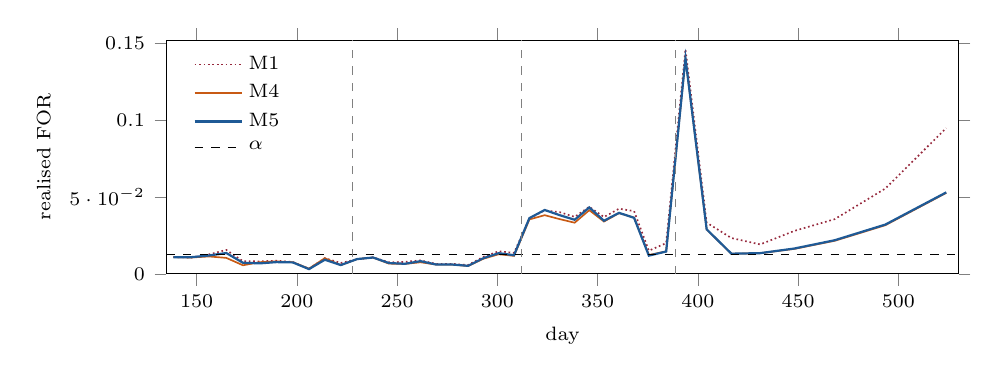
\begin{tikzpicture}
\begin{axis}[tinyplot, xlabel={day}, ylabel={realised FOR}, xmin=135, xmax=530,
  ymin=0, ymax=0.152, legend pos=north west, legend cell align=left]
\addplot[cD, densely dotted] coordinates {\SeriesMone};
\addlegendentry{M1}
\addplot[cB] coordinates {\SeriesMfour};
\addlegendentry{M4}
\addplot[cA, thick] coordinates {\SeriesMfive};
\addlegendentry{M5}
\addplot[black, dashed, line width=0.5pt] coordinates {(135,\AlphaSynb) (530,\AlphaSynb)};
\addlegendentry{$\alpha$}
\draw[gray, dashed] (axis cs:\DriftA,0) -- (axis cs:\DriftA,0.152);
\draw[gray, dashed] (axis cs:\DriftB,0) -- (axis cs:\DriftB,0.152);
\draw[gray, dashed] (axis cs:\DriftC,0) -- (axis cs:\DriftC,0.152);
\end{axis}
\end{tikzpicture}
\caption{Realised risk on released traffic, one point per block of 2000 transactions.
Vertical rules mark the covariate, concept and prior events. All three methods breach
$\alpha$ after the concept shift; only the spike height differs.}
\label{fig:series}
\end{figure}

%% Fig. 4 (budget-risk curve) cut for space; Table I carries per-method
%% capacity and the budget ablation is in the artefact.


\begin{figure}[t]
\centering
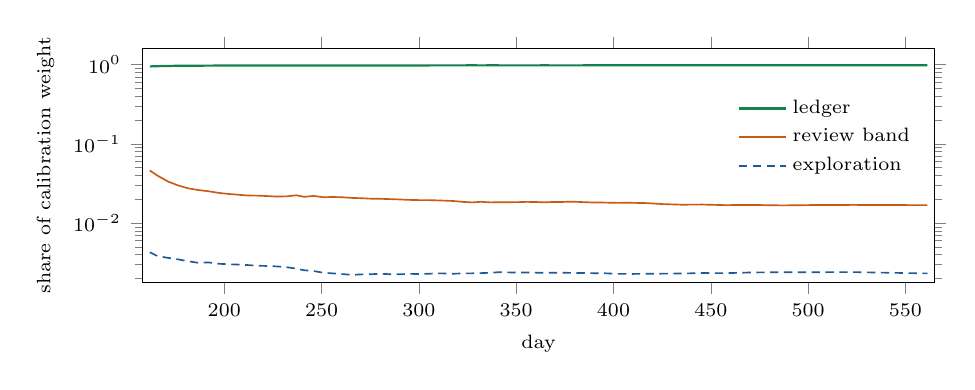
\begin{tikzpicture}
\begin{axis}[tinyplot, xlabel={day}, ylabel={share of calibration weight},
  xmin=158, xmax=565, ymode=log, ymin=0.0018, ymax=1.6,
  legend style={at={(0.98,0.62)}, anchor=east}, legend cell align=left]
\addplot[cC, thick] coordinates {\CompLedger};
\addlegendentry{ledger}
\addplot[cB] coordinates {\CompReview};
\addlegendentry{review band}
\addplot[cA, densely dashed] coordinates {\CompExplore};
\addlegendentry{exploration}
\end{axis}
\end{tikzpicture}
\caption{Where the calibration weight comes from, on a log scale. The review band, the
one channel whose labels are fast and correct, shrinks to under a fiftieth of the
window. This is the endogeneity, drawn.}
\label{fig:comp}
\end{figure}

\begin{table}[t]
\caption{Exploration ablation on SynB2B-Fraud-Stream under M5. Bias is the ratio of
true to estimated risk, with its bootstrap interval; $n_{\exp}$ counts explored items
over the evaluation stream.}
\label{tab:eps}
\centering\scriptsize
\setlength{\tabcolsep}{3.4pt}
\begin{tabular}{rrrlrrr}
\toprule
$\varepsilon$ & $n_{\exp}$ & Bias & 95\% CI & quiet FOR & hold & cost/1k\\
\midrule
\TableEpsBody
\bottomrule
\end{tabular}
\end{table}

Table~\ref{tab:eps} carries the exploration ablation. The trend is real, the step is
not: 0.866 [0.840, 0.893] at no exploration against 0.877 [0.854, 0.903] at 0.120 is a
gain of 0.011 with overlapping intervals, so most of the distance from M4's 0.0533
comes from the propensity correction rather than the 0.120, which was fixed as an
operating assumption before the ablation ran.

One ablation came out backwards. Set the delay multiplier to 0 so every label arrives
the instant the decision is taken, and the flag fires in 0.9988 of windows against
0.321 at the true delay, while realised risk improves to 0.019258. That is not perfect
feedback: undisclosed frauds are still booked clean at the close, so this removes the
delay alone. And removing it made the policy louder, not calmer. The lag was
concealing that the target could not be met at this capacity. Raising disclosure has a
related effect. At a multiplier of 2.4 the corrected ratio degrades from 0.877 to
0.660 while infeasibility climbs to 0.747.

Misses split by topology as disclosure does: wire redirection surfaces 0.86 of the
time and is missed at 0.0810, payment-term manipulation surfaces at 0.19 and is missed
at 0.671, and drift-induced fraud at 0.948, so the policy is blindest where the ledger
is quietest. Recovery takes 19.11 days after the covariate shift and never arrives
after the other two.

\begin{table}[t]
\caption{Cross-dataset transfer to the ULB card portfolio, $\alpha = 0.000930$.
Columns match Table~\ref{tab:methods}. The disclosure and delay layers are imposed by
us there too, so this tests portability across score and label distributions, not
across a real label-arrival system.}
\label{tab:ulb}
\centering\scriptsize
\setlength{\tabcolsep}{0.8pt}
\begin{tabular}{lrrrrrrr}
\toprule
Method & FOR & quiet & dem. & served & Infeas. & USD/1k & ratio\\
\midrule
\TableUlbBody
\bottomrule
\end{tabular}
\end{table}

Table~\ref{tab:ulb} reproduces the shape on a much rarer positive class and shows a
limit: M5 reaches a ratio of 0.903 where uncorrected M4 sits at 0.785, and the oracle
overshoots to 1.21, because that portfolio has no topology annotation and disclosure
depends on amount alone, leaving the propensity nearly flat and little for the
correction to undo. The method earns its keep where the disclosure law varies across
the population; where it does not, it costs 20.06 microseconds at p50 rather than 9.55
for nothing.

\section{Discussion and Threats to Validity}

The infeasibility rate is a result, not a defect, and it is where M5 wins outright.
The oracle searches every admissible threshold on the window's true risk curve and
calls it feasible if any clears $\alpha$, so it assumes no monotonicity. That matters:
(A2) does fail here, with 0.598 of admissible steps on M5's curve running downhill. It
changes nothing measurable. That oracle and Proposition~\ref{prop:feas} agree on 1.000
of scored windows. M5 reaches precision 0.924, recall 0.840 and balanced accuracy
0.898, ahead of M3 at 0.855 and M4 at 0.731, flagging 0.321 of windows against an
oracle rate of 0.348. M2's near-perfect recall of 0.999 comes of flagging 0.922 of
windows, leaving specificity at 0.119, while true risk in flagged windows is 0.02267
against 0.009543 in unflagged ones. M0 and M1 never update, so their zero is the
absence of a mechanism.

Practitioners treat label lag as a nuisance to be absorbed by a longer window. That is
wrong: a longer window admits more matured labels and more censored ones together, and
the censored ones carry a sign.

The limits below deserve to be stated plainly rather than softened. The drift was
injected by us, with magnitudes solved against targets we chose, so every recovery-
time number describes our generator and not any real payment network. The cost
constants are stipulated, which is why the cost column is reported and never argued
from. The propositions lean on (A1)--(A3), and monotonicity is the one a real portfolio
breaks first. And \eqref{eq:est} estimates an exponentially weighted risk on
the trimmed overlap population, not the trailing-window risk of
Section~\ref{sec:prob}, and we measure that gap rather than bound it.

The learned $p_d$ is not close either, missing the truth by 0.1566 on average on a
quantity that runs from 0.19 to 0.86, because the model sees amount and score and
never the fraud topology that actually sets disclosure, and handing it topology would
repair the number while voiding the experiment. It is fitted on the same censored
ledger it corrects, so a change of write-off policy moves $p_d$ with no signal in the
score distribution.

\section{Conclusion}

A budgeted fraud policy decides which labels it will ever receive, which makes its
calibration set a function of its own actions. We gave a feasibility condition for
when a target and a budget can coexist, and an identification result for what
exploration buys. The attached rate bound is vacuous at any operating point worth
running. What holds across two streams is
narrower than a theorem. Correcting for arrival propensity moves an estimator that
reads high by a factor of 19.3 to one that reads high by 13.5\%, for 0.120 of the
analyst budget and about nine microseconds per transaction. Realised risk is
unchanged, so the claim is a policy that can be audited, not one that is safer.

%% The acknowledgement was dropped for space: the licensing and artefact statement
%% it carried is already in Sec. V under the \ifanon toggle, so it was duplication.

\begin{thebibliography}{99}
\footnotesize

\bibitem{deng2026}
J. Deng, ``When can fraud operations authorize automation? A decision-support
framework for fresh audit evidence and review workload,'' arXiv:2608.08577, Aug. 2026.

\bibitem{vovk2005}
V. Vovk, A. Gammerman, and G. Shafer, \emph{Algorithmic Learning in a Random World}.
New York, NY, USA: Springer, 2005.

\bibitem{papadopoulos2002}
H. Papadopoulos, K. Proedrou, V. Vovk, and A. Gammerman, ``Inductive confidence
machines for regression,'' in \emph{Proc. 13th Eur. Conf. Mach. Learn. (ECML)},
Helsinki, Finland, 2002, pp. 345--356.

\bibitem{gibbs2021}
I. Gibbs and E. Cand\`es, ``Adaptive conformal inference under distribution shift,''
in \emph{Adv. Neural Inf. Process. Syst. (NeurIPS)}, vol. 34, 2021, pp. 1660--1672.

\bibitem{gibbs2024}
I. Gibbs and E. Cand\`es, ``Conformal inference for online prediction with arbitrary
distribution shifts,'' \emph{J. Mach. Learn. Res.}, vol. 25, no. 162, pp. 1--36, 2024.

\bibitem{angelopoulos2024}
A. N. Angelopoulos, S. Bates, A. Fisch, L. Lei, and T. Schuster, ``Conformal risk
control,'' in \emph{Proc. Int. Conf. Learn. Represent. (ICLR)}, Vienna, Austria, 2024.

\bibitem{bates2021}
S. Bates, A. Angelopoulos, L. Lei, J. Malik, and M. I. Jordan, ``Distribution-free,
risk-controlling prediction sets,'' \emph{J. ACM}, vol. 68, no. 6, pp. 1--34, 2021.

\bibitem{feldman2022}
S. Feldman, L. Ringel, S. Bates, and Y. Romano, ``Achieving risk control in online
learning settings,'' arXiv:2205.09095, 2022.

\bibitem{barber2023}
R. F. Barber, E. J. Cand\`es, A. Ramdas, and R. J. Tibshirani, ``Conformal prediction
beyond exchangeability,'' \emph{Ann. Statist.}, vol. 51, no. 2, pp. 816--845, 2023.

\bibitem{angelopoulos2023}
A. N. Angelopoulos, E. J. Cand\`es, and R. J. Tibshirani, ``Conformal PID control for
time series prediction,'' in \emph{Adv. Neural Inf. Process. Syst. (NeurIPS)},
vol. 36, 2023.

\bibitem{geifman2017}
Y. Geifman and R. El-Yaniv, ``Selective classification for deep neural networks,'' in
\emph{Adv. Neural Inf. Process. Syst. (NeurIPS)}, vol. 30, 2017, pp. 4878--4887.

\bibitem{geifman2019}
Y. Geifman and R. El-Yaniv, ``SelectiveNet: A deep neural network with an integrated
reject option,'' in \emph{Proc. Int. Conf. Mach. Learn. (ICML)}, Long Beach, CA, USA,
2019, pp. 2151--2159.

\bibitem{xu2024active}
Z. Xu, N. Karampatziakis, and P. Mineiro, ``Active, anytime-valid risk controlling
prediction sets,'' arXiv:2406.10490, Jun. 2024.

\bibitem{mozannar2020}
H. Mozannar and D. Sontag, ``Consistent estimators for learning to defer to an
expert,'' in \emph{Proc. Int. Conf. Mach. Learn. (ICML)}, 2020, pp. 7076--7087.

\bibitem{singh2026}
M. Singh, A. Srikantha, and S. Lakhanpal, ``Cost-sensitive conformal prediction and
human-in-the-loop abstention for imbalanced high-stakes decision support: A
multi-domain benchmark,'' arXiv:2607.27143, Jul. 2026.

\bibitem{xu2026}
Y. Xu, W. Guo, and Z. Wei, ``Selective conformal risk control,'' arXiv:2512.12844,
Dec. 2025, rev. Apr. 2026.

\bibitem{leong2026}
J. W. Leong, ``Online shift detection and conformal adaptation for deployed safety
classifiers,'' arXiv:2606.11949, Jun. 2026.

\bibitem{zhou2026}
Y. Zhou, R. Fathony, N. H. Nguyen, and M. Sesia, ``Audited conformal prediction for
classification under unknown distribution shift,'' arXiv:2606.14909, Jun. 2026.

\bibitem{hultberg2026}
B. Hultberg, D. Zachariah, and A. H. Ribeiro, ``Anytime-valid conformal risk
control,'' arXiv:2602.04364, Feb. 2026.

\bibitem{dalpozzolo2014}
A. Dal Pozzolo, O. Caelen, Y.-A. Le Borgne, S. Waterschoot, and G. Bontempi, ``Learned
lessons in credit card fraud detection from a practitioner perspective,'' \emph{Expert
Syst. Appl.}, vol. 41, no. 10, pp. 4915--4928, 2014.

\bibitem{dalpozzolo2018}
A. Dal Pozzolo, G. Boracchi, O. Caelen, C. Alippi, and G. Bontempi, ``Credit card
fraud detection: A realistic modeling and a novel learning strategy,'' \emph{IEEE
Trans. Neural Netw. Learn. Syst.}, vol. 29, no. 8, pp. 3784--3797, Aug. 2018.

\bibitem{dhama2026a}
G. Dhama, ``The fundamental limits of fraud detection in card payment networks,''
arXiv:2605.27557, May 2026.

\bibitem{dhama2026b}
G. Dhama, ``Causal label recovery in payment networks,'' arXiv:2605.29272, May 2026.

\bibitem{wang2026}
B. Wang, M. Zecchin, and O. Simeone, ``Online conformal prediction with corrupted
feedback,'' arXiv:2605.20515, May 2026.

\bibitem{lakkaraju2017}
H. Lakkaraju, J. Kleinberg, J. Leskovec, J. Ludwig, and S. Mullainathan, ``The
selective labels problem: Evaluating algorithmic predictions in the presence of
unobservables,'' in \emph{Proc. 23rd ACM SIGKDD Int. Conf. Knowl. Discovery Data
Mining}, Halifax, NS, Canada, 2017, pp. 275--284.

\bibitem{synb2b}
A. Sharma, ``SynB2B-Fraud: A synthetic dataset for fraud detection in B2B payment
networks,'' Zenodo, 2026, doi: 10.5281/zenodo.21668281.

\end{thebibliography}

\end{document}
